\documentclass[letterpaper,12pt]{article}
\usepackage{amsmath}  % improve math presentation
\usepackage{graphicx} % takes care of graphic including machinery
\usepackage{mathrsfs}


\usepackage[final]{hyperref} % adds hyper links inside the generated pdf file
\hypersetup{
	colorlinks=true,       % false: boxed links; true: colored links
	linkcolor=blue,        % color of internal links
	citecolor=blue,        % color of links to bibliography
	filecolor=magenta,     % color of file links
	urlcolor=blue         
}

\title{First Assignment for Computational Physics}
\date{\today}
\author{Xinyu Liu}



\begin{document}
\maketitle

\section{My Github Account}

My GitHub account is \textbf{rising1227}

\section{Self-Introduction}

    I'm a first year undergraduate student at NYU physics department. Before coming here, I had my undergrad at Tsinghua University in China.\\
    I've had some experience working on various programming languages(C++, python, Matlab, etc.), LaTeX and Github. During my undergraduate year, I've taken a course named big data in experimental physics where I learned essentially how experimentalists work. Also, I've conducted some theoretical research in hep-th and hep-ph which includes some application of solving PDE and ODE with programming languages.\\
    When I go to the graduate school, my research interest move from pure theoretical work towards aspects more on the intersection of theory and experiments. That's why I joined professor Emily's research group. I guess that my goal for this course is to familiar myself better with programming language. For right now, I'd like to explore more on physics and I would be really happy if I can explore further on physics after I graduate.




\newpage
\section{Including Graphics}

Here's the gaussian function that we've plotted with matplotlib\ref{plot}. The normalized gaussian function is:

\begin{equation}
    f(x) = \frac{1}{\sigma \sqrt{2\pi}} e^{-\frac{1}{2} (\frac{x-\mu}{\sigma})^2}
\end{equation}

\begin{table}[!h]
    \centering
    \caption{Gaussian function with $\sigma = 3$ and $\mu = 0$}
    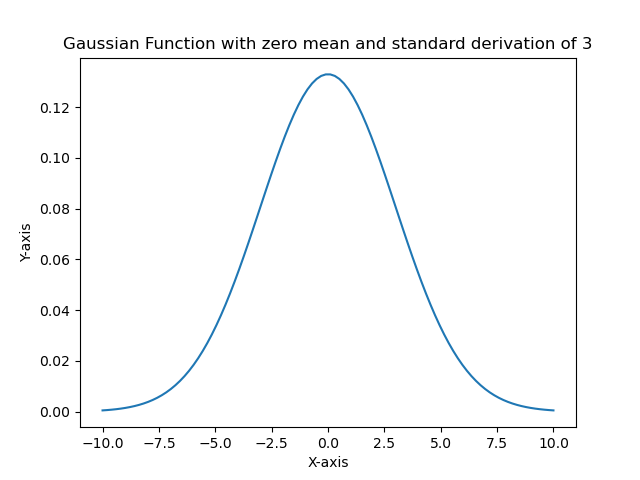
\includegraphics{gaussian.png}
    \label{plot}%
  \end{table}%





\end{document}